% !TeX spellcheck = en_GB
\documentclass[11pt]{article}
\usepackage{graphicx}
\usepackage{listings}
\usepackage[T1]{fontenc}
\graphicspath{
{./figures/}
}
\title{Machine Learning Project\\Task 3: Reinforcement Learning}
\author{Duy Nguyen Dinh \\ dinh@rhrk.uni-kl.de\and
	Minh Duc Duong\\ duong@rhrk.uni-kl.de\and
}
\date{\today}
\begin{document}

\maketitle

\section{Tabular Reinforcement Learning}

\subsection{Introduction to reinforcement learning}
Reinforcement learning is a type of learning, which results actions based on certain situation with the goal to maximize a specific value (reward signal). In the beginning, the model does not know what to do to maximize the reward but it must try to find out by itself through trials and errors. Each time the model try to learn the situation can either have the same parameters or affected by actions from the past learning, which is mentioned as delayed reward.

One of the problem of reinforcement learning is Markov decision process. This problem requires evaluate the outcome and choosing actions base on different situation to maximize the reward signal. The learner is called agent, which also makes decisions throughout the learning process. In this case, making decisions (actions) is interacting with things outside the agent, which is called environment. Each time the agent performs an action, depend on the current state s and the environment, it will move to another state s' and yield a reward R, which we want to maximize the cumulative sum overtime. The reward is simply a rational number and is the result of reward function, which evaluate the actions and is the driving force of how the agent should behave. For example, we have a robot as an agent with the objective to escape a maze with the minimum amount of steps. Then the return function will yield a negative reward as we want the agent to take less steps as possible.

Now from a certain time t, we have a sequence of reward for the next steps as R\textsubscript{t+1},  R\textsubscript{t+2} ... R\textsubscript{T}, where T is the final step. The sum of these numbers is called return. Also at the time t, the agent has a certain state s and we want to evaluate how good this current state, which is how much potential reward can we gain from this state in the future (return). This is done by using value functions. Value functions defined by the ways the agent behaves, which results in a certain number depends on the current state and the taken action. Policy is a mapping from states to probabilities of each possible actions. The notation is $\pi$(a$\vert$s), which is the probability the agent takes the action a if the current state is a. Thus the state-value function for Markov decision process can be defined as:

v\textsubscript{$\pi$}(s) = E\textsubscript{$\pi$}\big[ G\textsubscript{$t$}|S\textsubscript{t}=s \big] = E\textsubscript{$\pi$}\big[ $\sum_{k=0}^{\infty} \gamma^{k} R\textsubscript{t+k+1} | S\textsubscript{t}=s$ \big], for all s in S

where E\textsubscript{$\pi$}[$\bullet$] denoted as the expected value of random value given the time t and the policy $\pi$

We also define the value of taking action a in state s, denoted as q\textsubscript{$\pi$}(s$\vert$a).
This is action-value function for policy $\pi$

q\textsubscript{$\pi$}(s$\vert$a) = E\textsubscript{$\pi$}\big[ G\textsubscript{$t$}|S\textsubscript{t}=s,  A\textsubscript{t}=a \big] = E\textsubscript{$\pi$}\big[ $\sum_{k=0}^{\infty} \gamma^{k} R\textsubscript{t+k+1} | S\textsubscript{t}=s, A\textsubscript{t}=a $ \big]

For reinforcement learning, to maximize the return, we want to find the best policy at any given time. One policy can be better than the others. Its partial order can be defined using value function. If v\textsubscript{$\pi$}(s) >v\textsubscript{$\pi$'}(s) for all possible s, then $\pi$ is better than $\pi$'. Because there is one or more policies that are better than or equal to all others, these are optimal policy. If $\pi$ is an optimal policy, v\textsubscript{*}(s) is the optimal state-value function, which takes the maximum v\textsubscript{$\pi$}(s) of all possible states.

Aside from the case where the agent-environment interaction breaks into multiple subsequences (episodes), there are also the cases, which goes on infinitely. For such problem, we do not maximize the defined return but the discounted return:

G\textsubscript{t} = R\textsubscript{t+1} + $\gamma$R\textsubscript{t+2} + $\gamma^{2}$R\textsubscript{t+3} + ... with $0 \leq \gamma \leq 1$. Discount rate $\gamma$ decides the value of the future reward. As $\gamma$ less than 1, the further the reward the agent receives, the less relevant is the reward. As the discount rate gets closer to 1, the agent values the future reward more. We have a recursive formula for the discount return as G\textsubscript{t} = R\textsubscript{t+1} + $\gamma$G\textsubscript{t+1}. As the result, we need to maintain the consistency of the recursive formula for all policies and states. This leads to the Bellman equations as shown in the task sheet.

\subsection{Implementation and visualisation}

In this task, we don't make any changes in the \textit{gridworld.py}, the only extension is the implementation of new reward functions. The implementation of the required algorithms lies in the file \textit{tabular\_rl.py}.

The visualisation of movement in the gridworld was realized thanks to the library \textbf{gridworld-visualizer} \footnote{https://github.com/mvcisback/gridworld-visualizer} (We downloaded the source code and made some changes to adapt it). Since we haven't found any ways to put animating SVG files into PDF files yet, the movement figures are stored in the project (PATH: ./report/task3/figures/). These animating SVG files can be seen under a browser, or by the extension \textbf{SVG Viewer} in VS Code .

\subsection{SARSA}

in the SARSA algorithm, the lookup table Q is realized with a Numpy array in shape (16,16,4) (the dimensions of grid and number of actions combined). There are 5 hyperparameters: the number of episodes are executed, the probability of choosing a random action (or exploration rate), decay rate to reduce exploration rate, discount rate (step\_size), the maximum steps in an episode. We set the beginning exploration rate equals 1 and decay rate equals 0.99, so that it takes movement freely at the beginning and according to the policy later. The path the agent is consistent by over 2000 episodes (See PATH/sarsa\_path.svg). The best return of this method is roundly -35. The worst return is usually near the maximum steps (it is set to 100).

\includegraphics{sarsa_eps_return.pdf}

Next, we keep the exploring rate constantly and observe the behavior of the algorithm in different epsilon. According to the following figure, the number of success episodes over 1000 runs reduces dramastically when the epsilon increases. When epsilon equals 0, the agent moves in another way, which similar to one by the Q Learning algorithm. The reason of the difference lies on the way of choosing $A'$. When one always chooses the maximum $A'$, the agent is acknowledged about the margin of the Pits. Therefore, it will never step on the Pits and make zero negative impact backward the way (the SARSA did this). This is why the SARSA tries to avoid the region that has Pits.

\includegraphics{sarsa_succ_eps.pdf}

\subsection{Q Learning}

For the Q Learning, the path the agent is consistent by over 1000 episodes. It walks on another way from one with SARSA algorithm, because this algorithm has no fear with the Pits (See PATH/q\_learning\_path.svg). The best return of this mmethod is roundly -30, because the way near the Pits is shorter.

\includegraphics{q_learning_eps_return.pdf}

By comparing the plots, we can see that the Q-Learning has smaller impact from the epsilon than SARSA, because it chooses the random action once in a loop (the SARSA twice).

\includegraphics{q_learning_succ_eps.pdf}

\subsection{Reward functions}

As the task sheet required, we implemented 3 different value functions. 
\begin{itemize}
  \item The first value function indicates that the agent should find the shortest path to the goal while avoiding pits to maximize the reward. After a certain amount of episodes, we expect the agent to behave simply toward the goal, know how to avoid pits, swamps and arrows (most of the times) since these tile decrease the return.

  For the second value function, the agent will try to avoid pit and get to the goal. 

  The third function will make the agent as such, it keep leaning toward the direction of the tile goal while trying to avoid pit.

  \item As the problem required, the first value function should perform best compare to the other two.

  \item The second function does not get any penalty for each step (reward -1), which means the agent could reach the goal in one episode but can take a large number of steps. The path to the goal could not be optimal.

  The third function, while leaning toward goal cell can be a good thing. It does not aware of negative elements such as swamps and arrows. For example, in the given environment, the agent will keep going east direction. Like the second value function, this does not create an agent to solve the problem efficiently.
\end{itemize}

In this task, we use Q-Learning algorithm for experimenting the new reward functions. The hyperparameters are similar to task d.

For the second reward, we have no success episodes after 1000 runs. It seem like the lookup table never updates. After the agent reaches out the maximum step, it goes back to the start point, and the lookup table has no updates. Therefore, no success episode takes place.

\includegraphics{reward_2_q_learning_eps_return.pdf}

For the third reward, the agent reaches the goal as early as for the first reward. The behavior is also similar.We can notice that the maximum return is much lower (lower than -150), because the reward is Manhattan distant,which mostly smaller than -1.

\includegraphics{reward_3_q_learning_eps_return.pdf}

\subsection{Dynamic Programming: Value Iteration}

We realize Bellman optimality Equation by the Value Iteration algorithm, which outputs an optimal value function (instead of action-value function). The reson of this choice is the ability of visualisation. The action-value function can only be represented by a 3-dimensions array, which cannot easily find an appropriate visualisation approach. Value function can be described with a 2-d array instead, so we can use the heatmap model to observe each iteration. The following figures show the result of Value Iteration with different reward functions:

\includegraphics{value_iter_reward_1.pdf}

\includegraphics{value_iter_reward_2.pdf}

\includegraphics{value_iter_reward_2_discount_09.pdf}

\includegraphics{value_iter_reward_3.pdf}

We can easily generate the policy for each value function (always choose the direction with maximum reward value). For the first and third reward, we can draw a path from the start to the goal, according to the generated policy. One thing to emphasize is the number of iterations: the algorithm runs with the first reward converged after 77 iterations, with third reward 329 iterations.

The discount rateaffects the speed in this algorithm. The smaller discount, the faster the iteration converges. On the other hand, we have to sure that the convergence criteria doesn't meet, until the message propagation from the goal reaches the start. One interesting thing he have to pay attention: The algorithm runs with the second reward works only, when the discount rate is smaller than 1 (greater than 1 leads to divergence). When discount equals 1, the whole map (enterable states) has value 1.  

\section{Q-Learning For Cart Pole Problem}

For problems which have infinite number of states such as Cart-pole problem, we can either discrete the parameters for states or implement with deep neural network.

\subsection{Discretization}

In this task, we have to find a proper way to discretize the state space of the cart pole problem. The state space consists of 4 dimensions: the position, the velocity, the angel (theta), the angel velocity. According to the environment, the position bounds are -2.4 and 2.4, angel bounds -12 degree and 12 degree, the velocity has no bounds. Since we have only size-limited arrays, we need to set some suitable bounds for the velocity by setting default bounds and continuously extending these when the out-of-bound exception occures.

A critical parameter for the learning process is the number of buckets (for each dimension). For large numbers of buckets, the learning process will slow down and perform worse, because not all record in the policy array can be covered. Therefore, we set the number of buckets for each dimensions to 4.

Next, we can choose only a subset of dimensions to perform the learning. We found out that the subset consists of theta and theta velocity outperforms other subsets.

We optimize also the exploration rate of the algorithm: The return of episodes will be recorded, then calculate the average of returns last 5 episodes. Then the exploration rate $er = max(0, 1 - last_scores_avg / 40)$.  This means, the exploration rate is getting smaller, when the last score average bigger. Until the last score average bigger than 40 (we can tune this parameter), then the exploration phase is over.

\begin{lstlisting}[language=python, caption=distance functions]
last_scores = eps_scores[-5:]
last_scores_avg = sum(last_scores) / max(1,len(last_scores))
er = max(0, 1 - last_scores_avg / 40)
\end{lstlisting}

The plot below shows the result of this work. After over 50 episodes, the cart pole performs better. It gets more than 100 steps each episode. The requirement of solving the problem cannot not meet despite tuning the parameters (number of buckets, subset of dimensions, exploration mechanism).

\includegraphics{discretize_theta.pdf}

\subsection{Deep Q-Learning}

We implement a neural network with 4 x 32 x 2 with the learning rate of 1e-3, Adam optimizer, loss function MSE. As we are dealing with problem with infinite number of states, we also have a discount rate less than 1 (0.99). The probability of choosing random action is 1 at the beginning and start to rely more on the Q value later into the training.

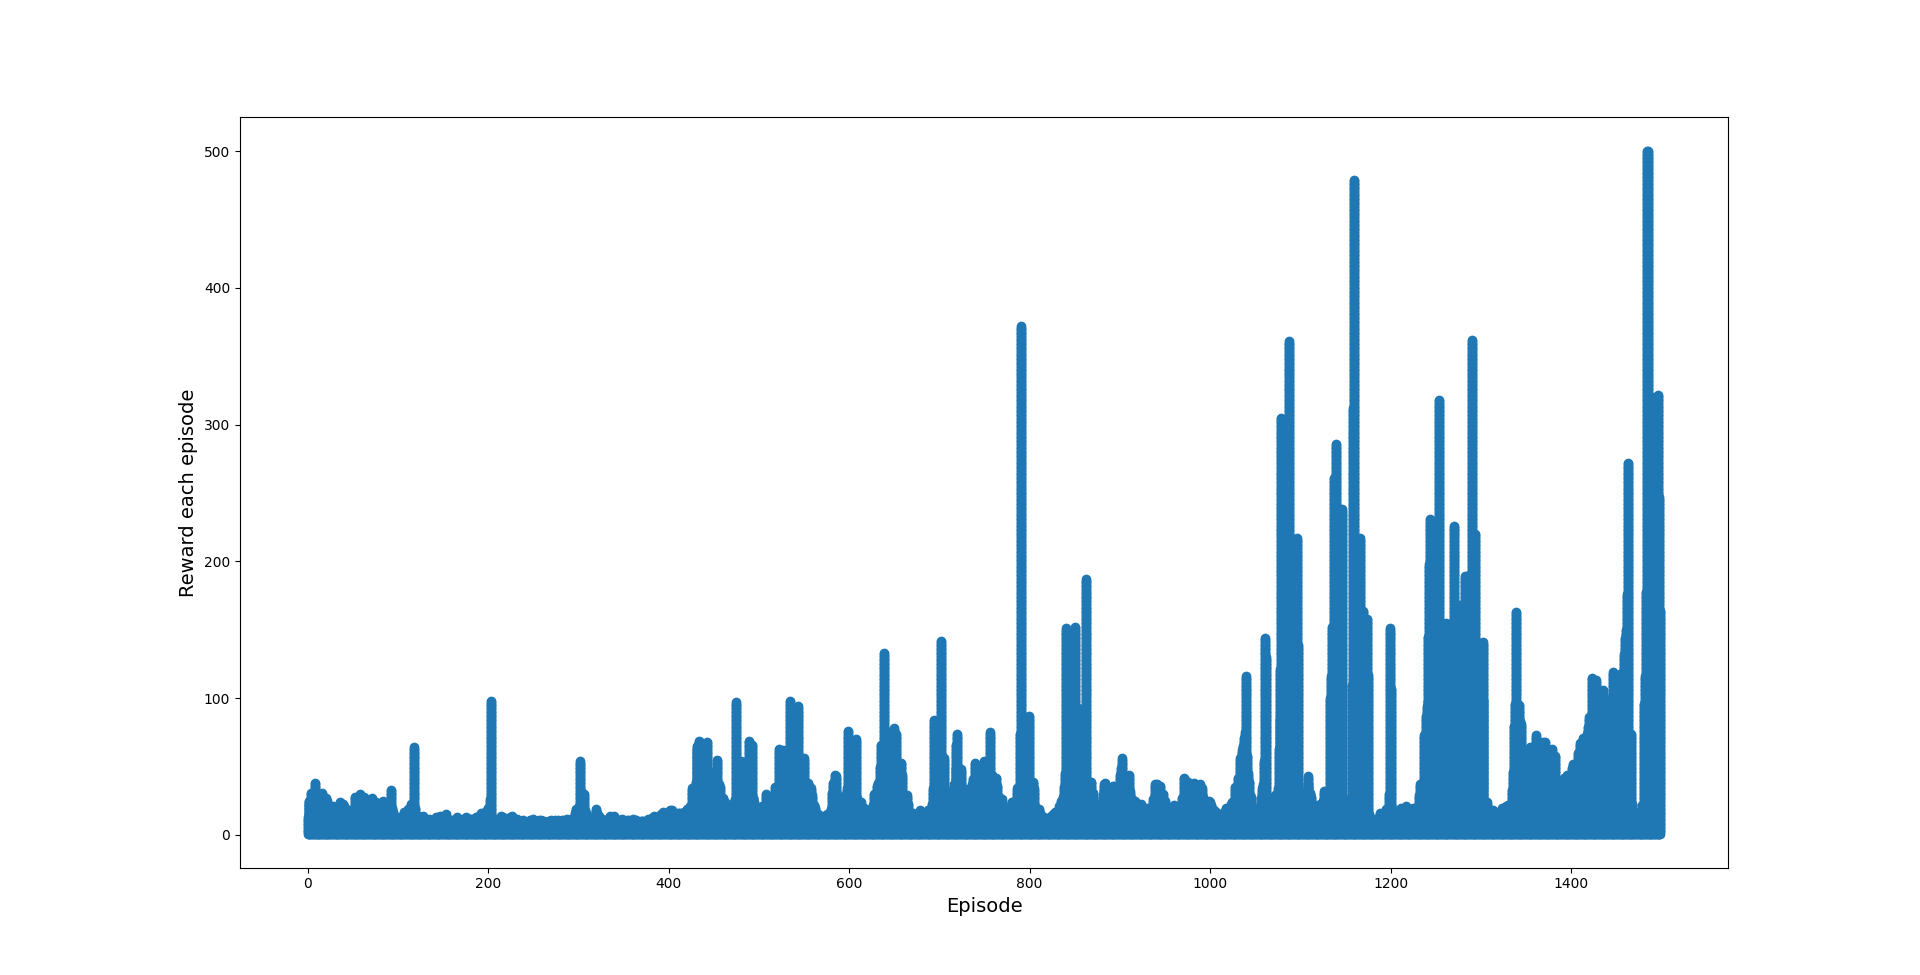
\includegraphics[width=\textwidth,height=\textheight,keepaspectratio]{figures/dqn.png}

The implementation can be found in cartpole\_dqn.py. We train the model with 1500 episodes. The result is inconsistent. After 200 episodes, the reward exceeds over 100 for the first time, but is very low for the most episodes. As later into training, the reward keep getting better but still very low most of the time.

At this point, parameters tuning is necessary. The result how ever give us no indication of which parameters should we change. Thus we decided to increase the size of the network by adding another hidden layer with 64 nodes (4 x 32 x 64 x 2). As we expect for a better result, we decrease the number of episodes to 750.

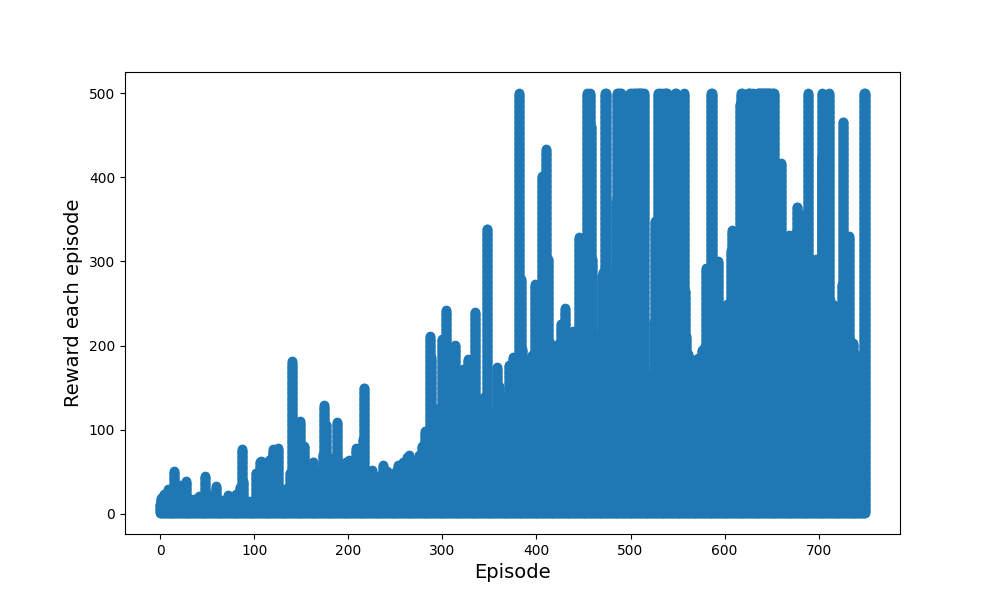
\includegraphics[width=\textwidth,height=\textheight,keepaspectratio]{figures/dqn2.png}

The model get to reward 100 in a single episode faster (after about 150 episodes). After about 400 episodes, the training agent keep getting the reward over 100 and most of the time peak at 500, which is good. However, there is a huge different between its lowest and its highest (even at the time when reward still exceeds over 100 at its low), which still proved the point mentioned in the task sheet, which is training the agent in deep neural network with Q-Learning is still unstable.

To make this point clearer, we training the agent again.

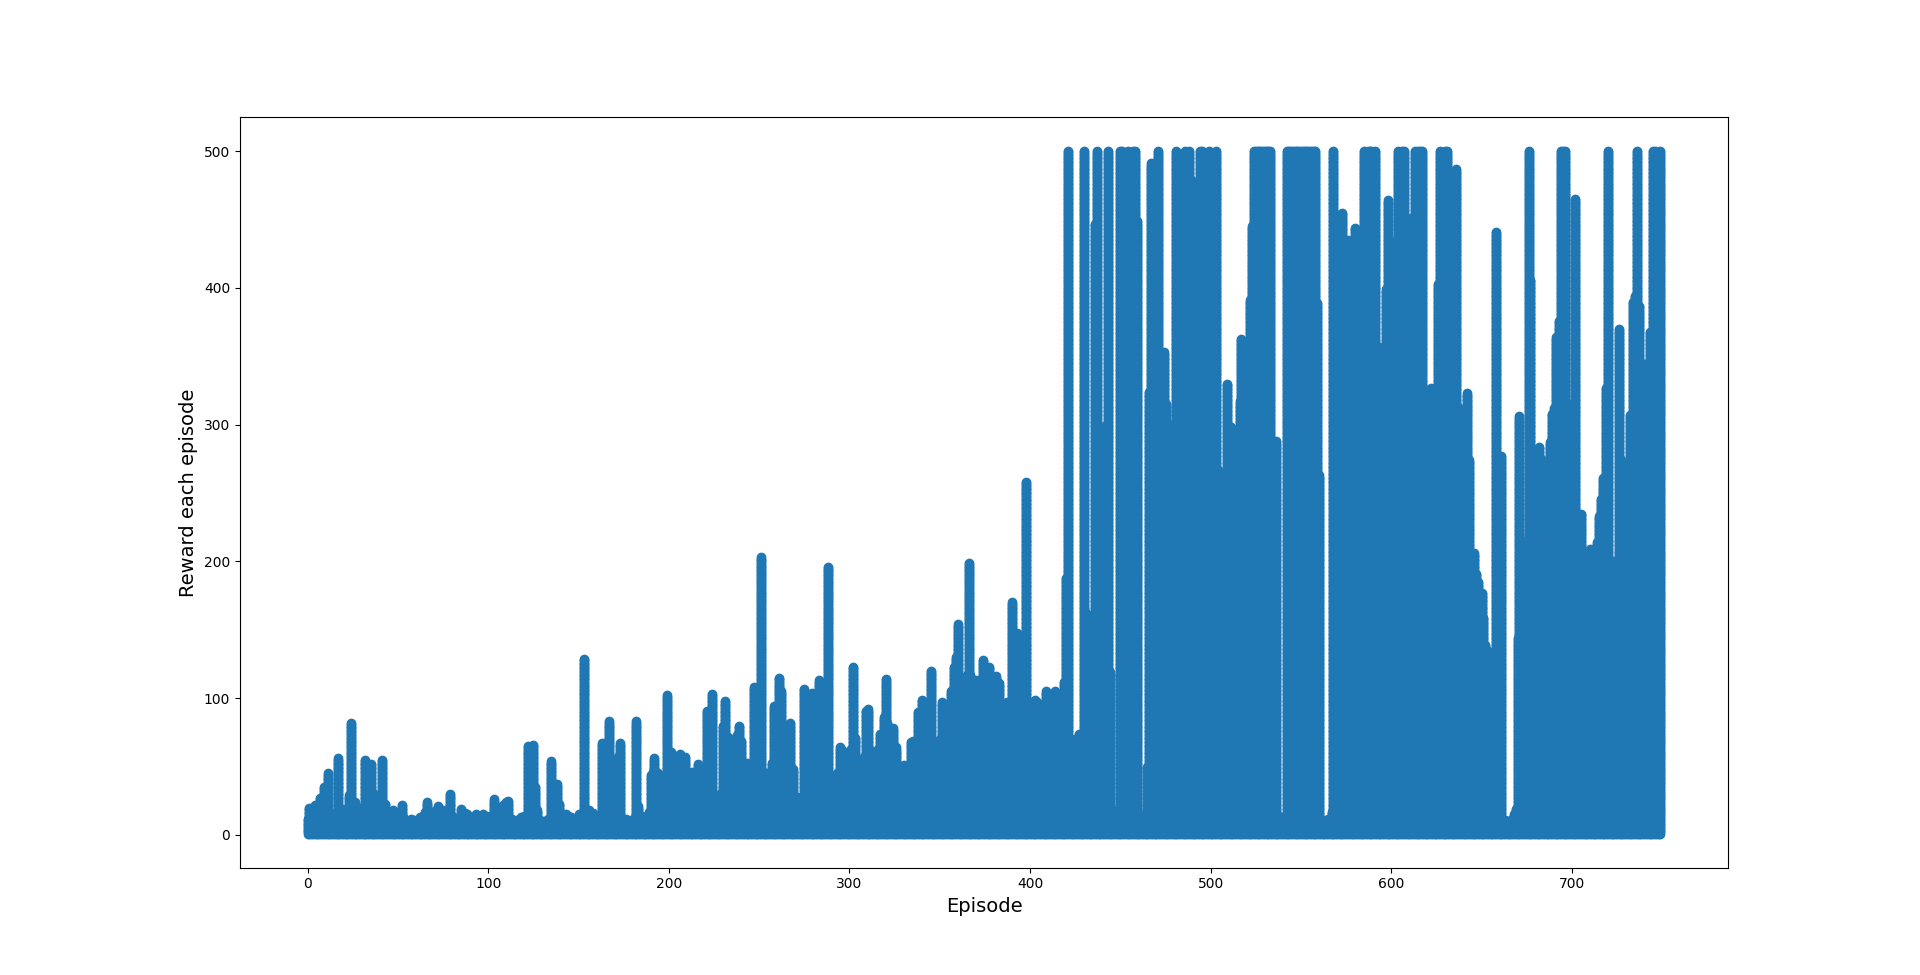
\includegraphics[width=\textwidth,height=\textheight,keepaspectratio]{figures/dqn3.png}

Even after 400 episodes, at its lowest, the reward can get very close to 0 and under 100 many times. In other word, it can still fail at solving the problem anytime after many episodes. Not to mentioned, all of these results  do not meet the requirement mentioned in the task sheet (though keep changing numbers through trials and errors can do but does not fix the inconsistency), which is why further modification is needed.

\subsection{Deep Q-Learning With Experience Replay}

The implementation can be found in cartpole\_dqn\_eb.py. As the task sheet recommend, we add an experience replay buffer to improve the model. The buffer has the size of 10000, and each time we train the model, we sample 128 tuples. When the buffer is full and another tuple will be added, we add it and remove the oldest one from the buffer. The hyper-parameters of the model is the same as the one in the last section.

We start with a network of 4 x 32 x 2

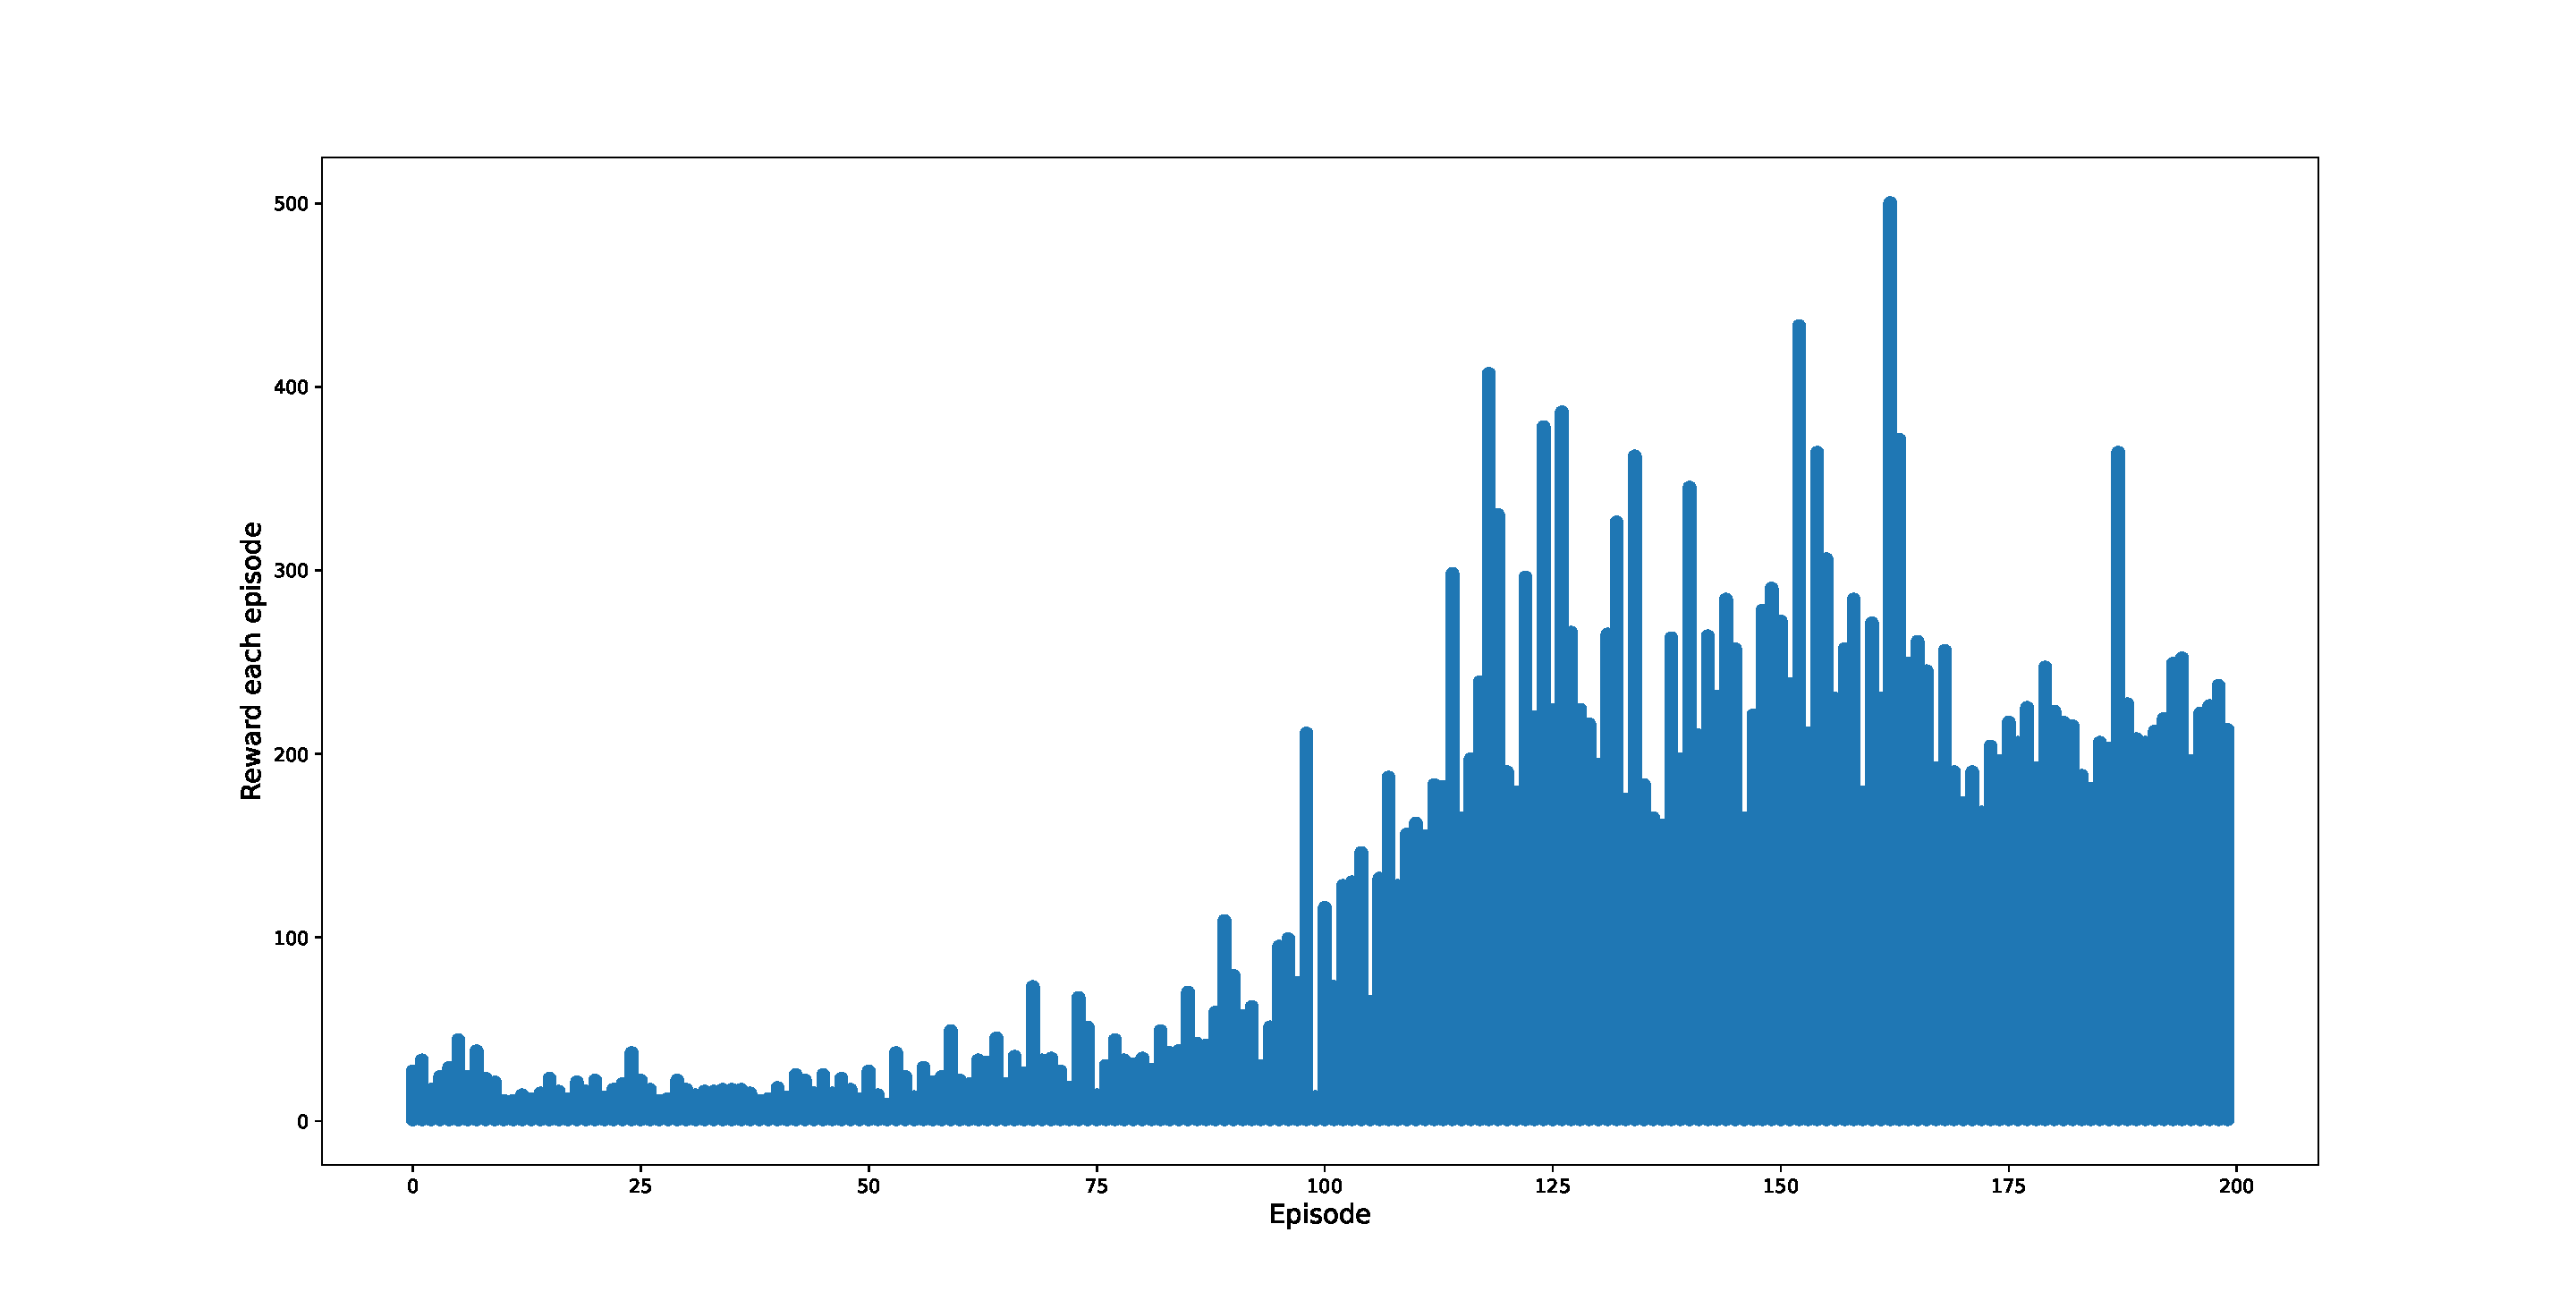
\includegraphics[width=\textwidth,height=\textheight,keepaspectratio]{figures/dqn_buffer.pdf}

The result shown a significant improvement. We only use 200 episodes and the reward exceeds 100 consistently after less than 100 episodes. The peak reward also grow faster compare to the previous approach without a buffer.

This defined network does solve the given problem in the task sheet. Furthermore, we still want to check for the consistency. For this, we use a bigger network (4 x 32 x 64 x 2) and 500 episodes (to see the actual returns in a long run).

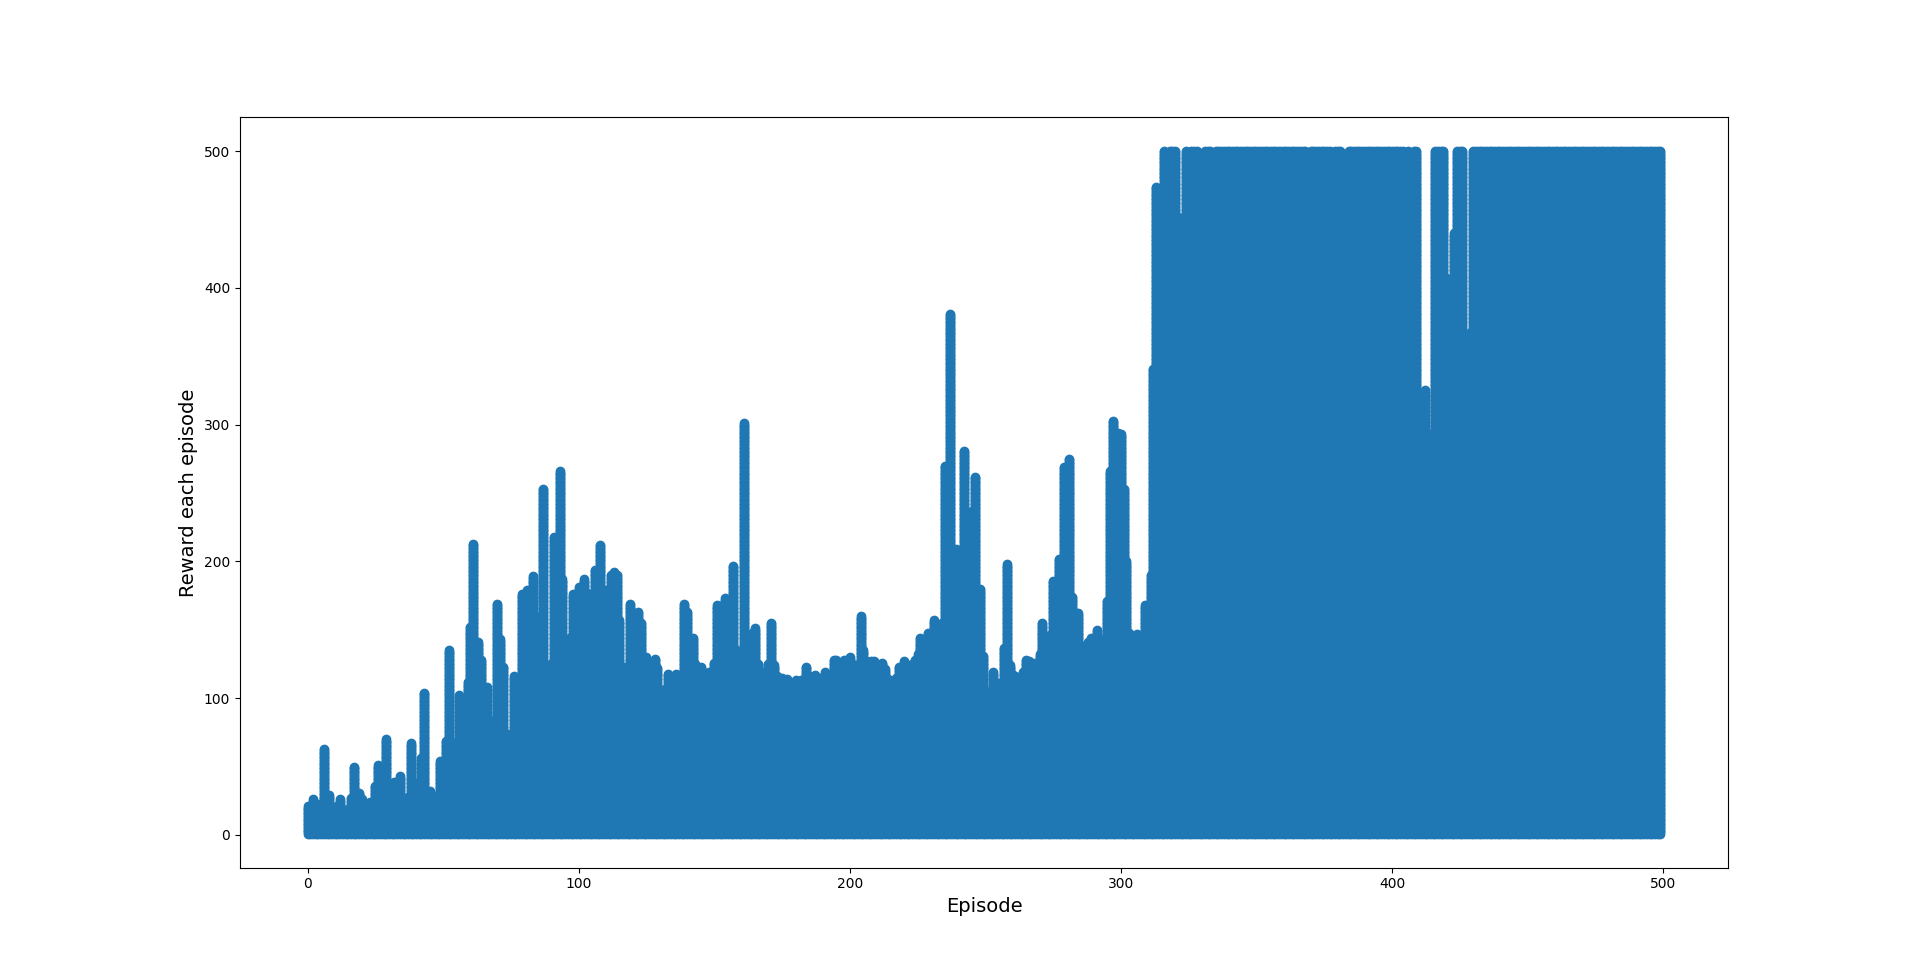
\includegraphics[width=\textwidth,height=\textheight,keepaspectratio]{figures/dqn_buffer2.png}

After over 300 episodes, the rewards are peak at 500 most of the times with a few exceptions (which are still over 100). The discrepancy between lowest and highest also much smaller compare to the previous implementation. We can come to the conclusion that using experience buffer does solve the issue with consistency.

This report used reference from Sutton and Barto and \href{https://pytorch.org/tutorials/intermediate/reinforcement_q_learning.html}{Reinforcement Learning (DQN) Tutorial from Pytorch documentation}


% Print references
\end{document}
